\section{Integrationstheorie}
\subsection{Integration einer positiven Funktion $f > 0$}
	  Für $s: R^d \rightarrow [0,\infty)$ mit 
	  \begin{equation}
	  	s =\ssum \alpha_k \textsl{x}{x}_k \qquad \alpha_{A_k} \neq 0
	  \end{equation}	   
	  ist das Integral gegeben durch
	  \begin{equation}
	  	\int s\; dx = \ssum \alpha_k v_d(A_k) \leq \infty
	  \end{equation}
	  Der Wert $\infty$ tritt immer nur dann auf, wenn $v_d(A_k) = \infty$ und $\alpha_k > 0$. Es folgt
	  \begin{equation}
	  	v(E) = \int \textsl{x}{x}_E dx
	  \end{equation}
	  Das Integral einer Funktion $f:R^d \to \R,\; f \geq 0$ ist definiert durch
	  \begin{equation}
	  	\int f\;dx := \lim_{n \to \infty} \int s_n dx \leq \infty 
	  \end{equation}
	  	wobei mit $s_n \leq s_{n+1} \leq ...  \quad s_n \to f$ (siehe Satz \ref{th:leb_elem_folg}) 
	  \begin{equation}
	   	\int_E f \;dx := \int \textsl{x}_E f \; dx
	  \end{equation}
	   gilt.
	  \begin{satz}
	   	Für jede Funktion $f \geq 0$ gilt
	   	\begin{equation}
	   		v(E) = 0 \Rightarrow \int_E f \; dx = 0
	   	\end{equation}
	   \end{satz}
	   
	   \subsection{Monotone Konvergenz}
	   \begin{satz} Satz über monotone Konvergenz \newline
	   Ist $f \geq 0$ und $0 \leq f_n \leq f_{n+1} \leq ... \leq f$ mit $f_n(x) \to f(x)$ fast überall, dann gilt
	   \begin{equation}
	   	\int_E f \;dx = \lim_{n \to \infty} \int_E f_n \;dx \leq \infty
	   \end{equation}
	   	(wobei fast überall überall bis auf eine Nullmenge meint).
	   \end{satz}
	   \begin{bsp}
	   	\begin{align*}
	   	\int_{[1,\infty]} \frac{1}{x}\; dx = \lim_{n \to \infty} \int_1^n \frac{1}{x} \; dx
	   	\end{align*}
	   \end{bsp}
	  
	  \subsection{Integrierbare Funktionen}
	  Eine Funktion $f: E \to \R$ heißt integrierbar wenn (analog zur absoluten Konvergenz bei Reihen siehe HM1)
	  \begin{equation}
	  	\int_E |f| \; dx < \infty
	  \end{equation}
	  gilt. Weiterhin ist 
	  \begin{equation}
	  	\int_E f\; dx := \int_E f_+ dx -\int_E  f_- dx \qquad \in \R
	  \end{equation}
	  wobei folgende Zusammenhänge gelten
	  \begin{align}
	  	f_+ (x) &= \max \lbrace f(x),0 \rbrace  \geq 0\\
	  	f_- ( x) &= \max \lbrace -f(x),0 \rbrace  \geq 0\\
	  	f(x) &= f_+(x) - f_-(x) \\
	  	|f(x)| &= f_+(x) + f_-(x)
	  \end{align}
	  und damit gilt auch:
	  \begin{equation}
	  	\int f_\pm \; dx \leq f \int |f| \;dx < \infty
	  \end{equation}
	  
	  \subsection{Eigenschaften des Integrals}
	  Seien $f,g:E \to \R$ integrierbar und $\alpha, \beta \in \R$. Dann gelten folgende Eigenschaften:
	  \begin{description}
		  \item[1) ]
	  	  \begin{equation}
	  		\int_E (\alpha f + \beta g)\;dx = \alpha \int_E f\;dx + \beta \int_E g \; dx
	  	  \end{equation}
		  \item[2) ]
		  \begin{equation}
		  	f \leq g \Rightarrow \int_E f \dx \leq \int_E g \dx
		  \end{equation}
		  \item[3) ]
		  \begin{equation}
		  	\left|\int_E f\dx\right| \leq \int_E |f| \dx
		  \end{equation}
		  \item[4) ]
		  \begin{equation}
		  	v(E) = 0 \Rightarrow \int_E f\dx = 0
		  \end{equation}
		  \item[5) ]
		  \begin{equation}
		  	v(E_1 \cap E_2) = 0 \Rightarrow \int_{E_1 \cup E_2} f \dx = \int_{E_1}f\dx + \int_{E_2}f\dx
		  \end{equation}
		  \item[6) ]
		  \begin{equation}
		  	f(x) = g(x) \text{ (fast überall) } \Rightarrow \int_E f\dx = \int_E g\dx
		  \end{equation}
		  \item[7) ]
		  Fallls $|f_n| \leq |f|$ und $f_n(x) \to f(x)\;(n \to \infty)$ fast überall, dann gilt
		  \begin{equation}
		  	\int_E f(x) \dx = \lim_{n \to \infty} \int_E f_n \dx
		  \end{equation}
	  \end{description}
	  \begin{satz} Satz von Lebesgue über majorisierte Konvergenz \newline
	  Sei $f_n: E \to \R$ eine Folge von Funktionen mit $\lim_{n \to \infty} f_n(x) = f(x)$ fast überall. Falls $g>0$ existiert mit $\int g\dx < \infty$ und $|f_n| \leq \; g \forall n$, dann ist $f$ integrierbar und 
	  \begin{equation}
	  	\int_E f \dx = \lim_{n \to \infty} \int_E f_n \dx
	  \end{equation}	   	  
	  \end{satz}
	  
	  \subsection{Grundlegende Sätze zur Integration}
	  \subsubsection{Satz von Fubini}
	  \begin{definition}
	  	Lebesgue-integrierbare Funktionen \newline
	  	Für ein Gebiet $D\subset \R^n$ ist die Menge $L\uparrow(D)$ die Menge derjenigen Funktionen, die fast überall in $D$ Grenzwert einer monoton wachsenden Folge von Treppenfunktionen $(\varphi_k)$ sind und für die die Folge $(\int_D \varphi_k(\vec{x}) d\vec{x})$ konvergiert. Für $f \in L \uparrow (D)$ ist 
	  	\begin{equation}
	  		\int_D f(\vec{x}) d\vec{x} = \lim_{k \to \infty} \int_D \varphi_k(\vec{x}) d\vec{x}
	  	\end{equation}
	  	Die Menge $L\uparrow(D)$, definiert durch
	  	\begin{align}
	  		L(I) &= L\uparrow(D) - L \uparrow (D) \nonumber \\
	  		&= \lbrace f = f_1 - f_2 : f_1, f_2 \in L \uparrow (D) \rbrace 
	  	\end{align}
	  	heißt die Menge der Lebesgue-integrierbaren Funktionen über $D$. Für $f \in L(D)$ ist das Integral definiert durch:
	  	\begin{equation}
	  		 \int_D f(\vec{x})\; d\vec{x} = \int_D f_1(\vec{x})\;d\vec{x} - \int_D f_2(\vec{x})\;d\vec{x}
	  	\end{equation}
	  \end{definition}
	  
	  \begin{satz}
	  	Satz von Fubini \newline
	  	Sind $I \subset \R$ und $J\subset \R^p$ (möglicherweise unbeschränkte) Quader sowie $f \in L(Q)$ eine auf dem Quader $Q = I \times J \subset \R^{p+q}$ integrierbare Fuktion, so gibt es Funktionen $g \in L(I)$ und $h \in L(J)$ mit 
	  	\begin{align}
	  		g(\vec{x}) &= \int_J f(\vec{x}, \vec{y}) \;d\vec{y} \qquad f.f.a. \; \vec{x} \in I,\\
	  		h(\vec{y}) &= \int_I f(\vec{x}, \vec{y}) \; d\vec{x} \qquad f.f.a \; \vec{y} \in J
	  	\end{align}
	  	Wobei mit f.f.a. für fast alle gemeint ist.
	  	Ferner ist
	  	\begin{align}
	  		\int_R f(\vec{x}, \vec{y}) \;d(\vec{x},\vec{y}) &= \int_I \int_J f(\vec{x}, \vec{y})\;d\vec{y} d\vec{x} = \int_I g(\vec{x}) \;d\vec{x} \nonumber \\
	  		&= \int_J\int_I f(\vec{x}, \vec{y})\; d\vec{x} d\vec{y} = \int_J h(\vec{y}) \;d\vec{y}
	  	\end{align}
	  \end{satz}
	  
	  \begin{bem}
	  	Mit dieser Formulierung werden sämtliche Dimensionen abgedeckt. Letztendlich besagt der Satz von Fubini aber, dass sich Gebietsintegrale über Quader immer als iterierte Integrale über einzelne Koordinaten berechnen lassen wobei die Integrationsreihenfolge egal ist.
	  \end{bem}
	  
	  \begin{satz}
	  Satz von Fubini: Spezialfall Quader\newline
	  Sei $Q = [a,b] \times [c,d] \subset \R^2$ und sei $f:G \to \R$ stetig, dann gilt
	  \begin{equation}
	  	\int_Q f(x,y) d(x,y) = \int_a^b \dx \int_c^d \dy f(x,y) = \int_c^d \dy \int_a^b \dx f(x,y)
	  \end{equation}
	  \end{satz}
	  
	  \begin{satz}
	  	Satz von Fubini und Torelli \newline
	  	Sei $E \subset \R^n \times \R^m$ und sei $f:E \to \R$ integrierbar oder positiv. Dann gilt
	  	\begin{align}
	  		\int f(x,y)\; d(x,y) &= \int_{\R^n} \dx \int_{E_x} \dy  \; f(x,y) \nonumber \\
	  		&= \int_{\R^m} \dy \int_{E^y} \dx  \; f(x,y)
	  	\end{align}
	  	wobei
	  	\begin{align}
	  		E_x &= \lbrace y | (x,y) \in E \rbrace \subset \R^m \nonumber \\
	  		E^y &= \lbrace x | (x,y) \in E \rbrace \subset \R^n \nonumber
	  	\end{align}
	  \end{satz}
	  
	  \subsubsection{Integrationsbereiche}
	  \begin{definition}
	  Normalbereiche: \newline
	  \textbf{Allgemein}: Es existiert ein Intervall $I$ und Funktionen $g_j,h_j:\R^j \to \R;\;j=1, ..., n-1$ sodass
	  \begin{align}
	  	D = \lbrace \vec{x} \in \R^n | x_1 \in I, \nonumber \\
	  		g_1(x_1) \leq x_2 &\leq h_1(x_1) \nonumber \\
	  		g_2(x_1, x_2) \leq x_3 &\leq h_2(x_1,x_2) \nonumber \\
	  		\dots \nonumber \\
	  		g_{n-1}(x_1,...,x_{n-1} \leq x_n &\leq h_{n-1}(x_1, ..., x_{n-1}) \rbrace
 	  \end{align}
 	 \textbf{ Im $R^2$}: $E \subset \R^2$ heißt Normalbereich vom Typ $I$, wenn die Zahlen $a,b \in \R$ und $C^0$-Funktionen $g,h:[a,b]\to \R$ existieren mit
 	 \begin{equation}
 	 	E = \lbrace (x,y) | a \leq x \leq b, \;g(x) \leq y \leq h(x) \rbrace
 	 \end{equation}
 	 Nach Fubini gilt dann:
 	 \begin{equation}
 	 	\int_E f\; d(x,y) = \int_a^b \dx \int_{g(x)}^{h(x)} \dy \; f(x,y)
 	 \end{equation}
 	 Ein Normalbereich vom Typ $II$ hat die Form 
 	 \begin{equation}
 	 	E = \lbrace (x,y) | c \leq y \leq d,\; l(y) \leq x \leq r(x)\rbrace
 	 \end{equation}
 	 und es gilt :
 	 \begin{equation}
 	 	\int_E f\; d(x,y) = \int_c^d \dy \int_{l(x)}^{r(x)} \dx \; f(x,y)
 	 \end{equation}
 	 \newline
 	 Anders formuliert: \newline
 	 \textbf{Normalbereich Typ $I$}
 	 \begin{equation}
 	 	B:= \lbrace (x,y) \in \R^2| a \leq x \leq b,\; \varphi_1(x) \leq y \leq \varphi_2(x)\rbrace
 	 \end{equation}
	  \begin{figure}[H] 
		  \centering
		  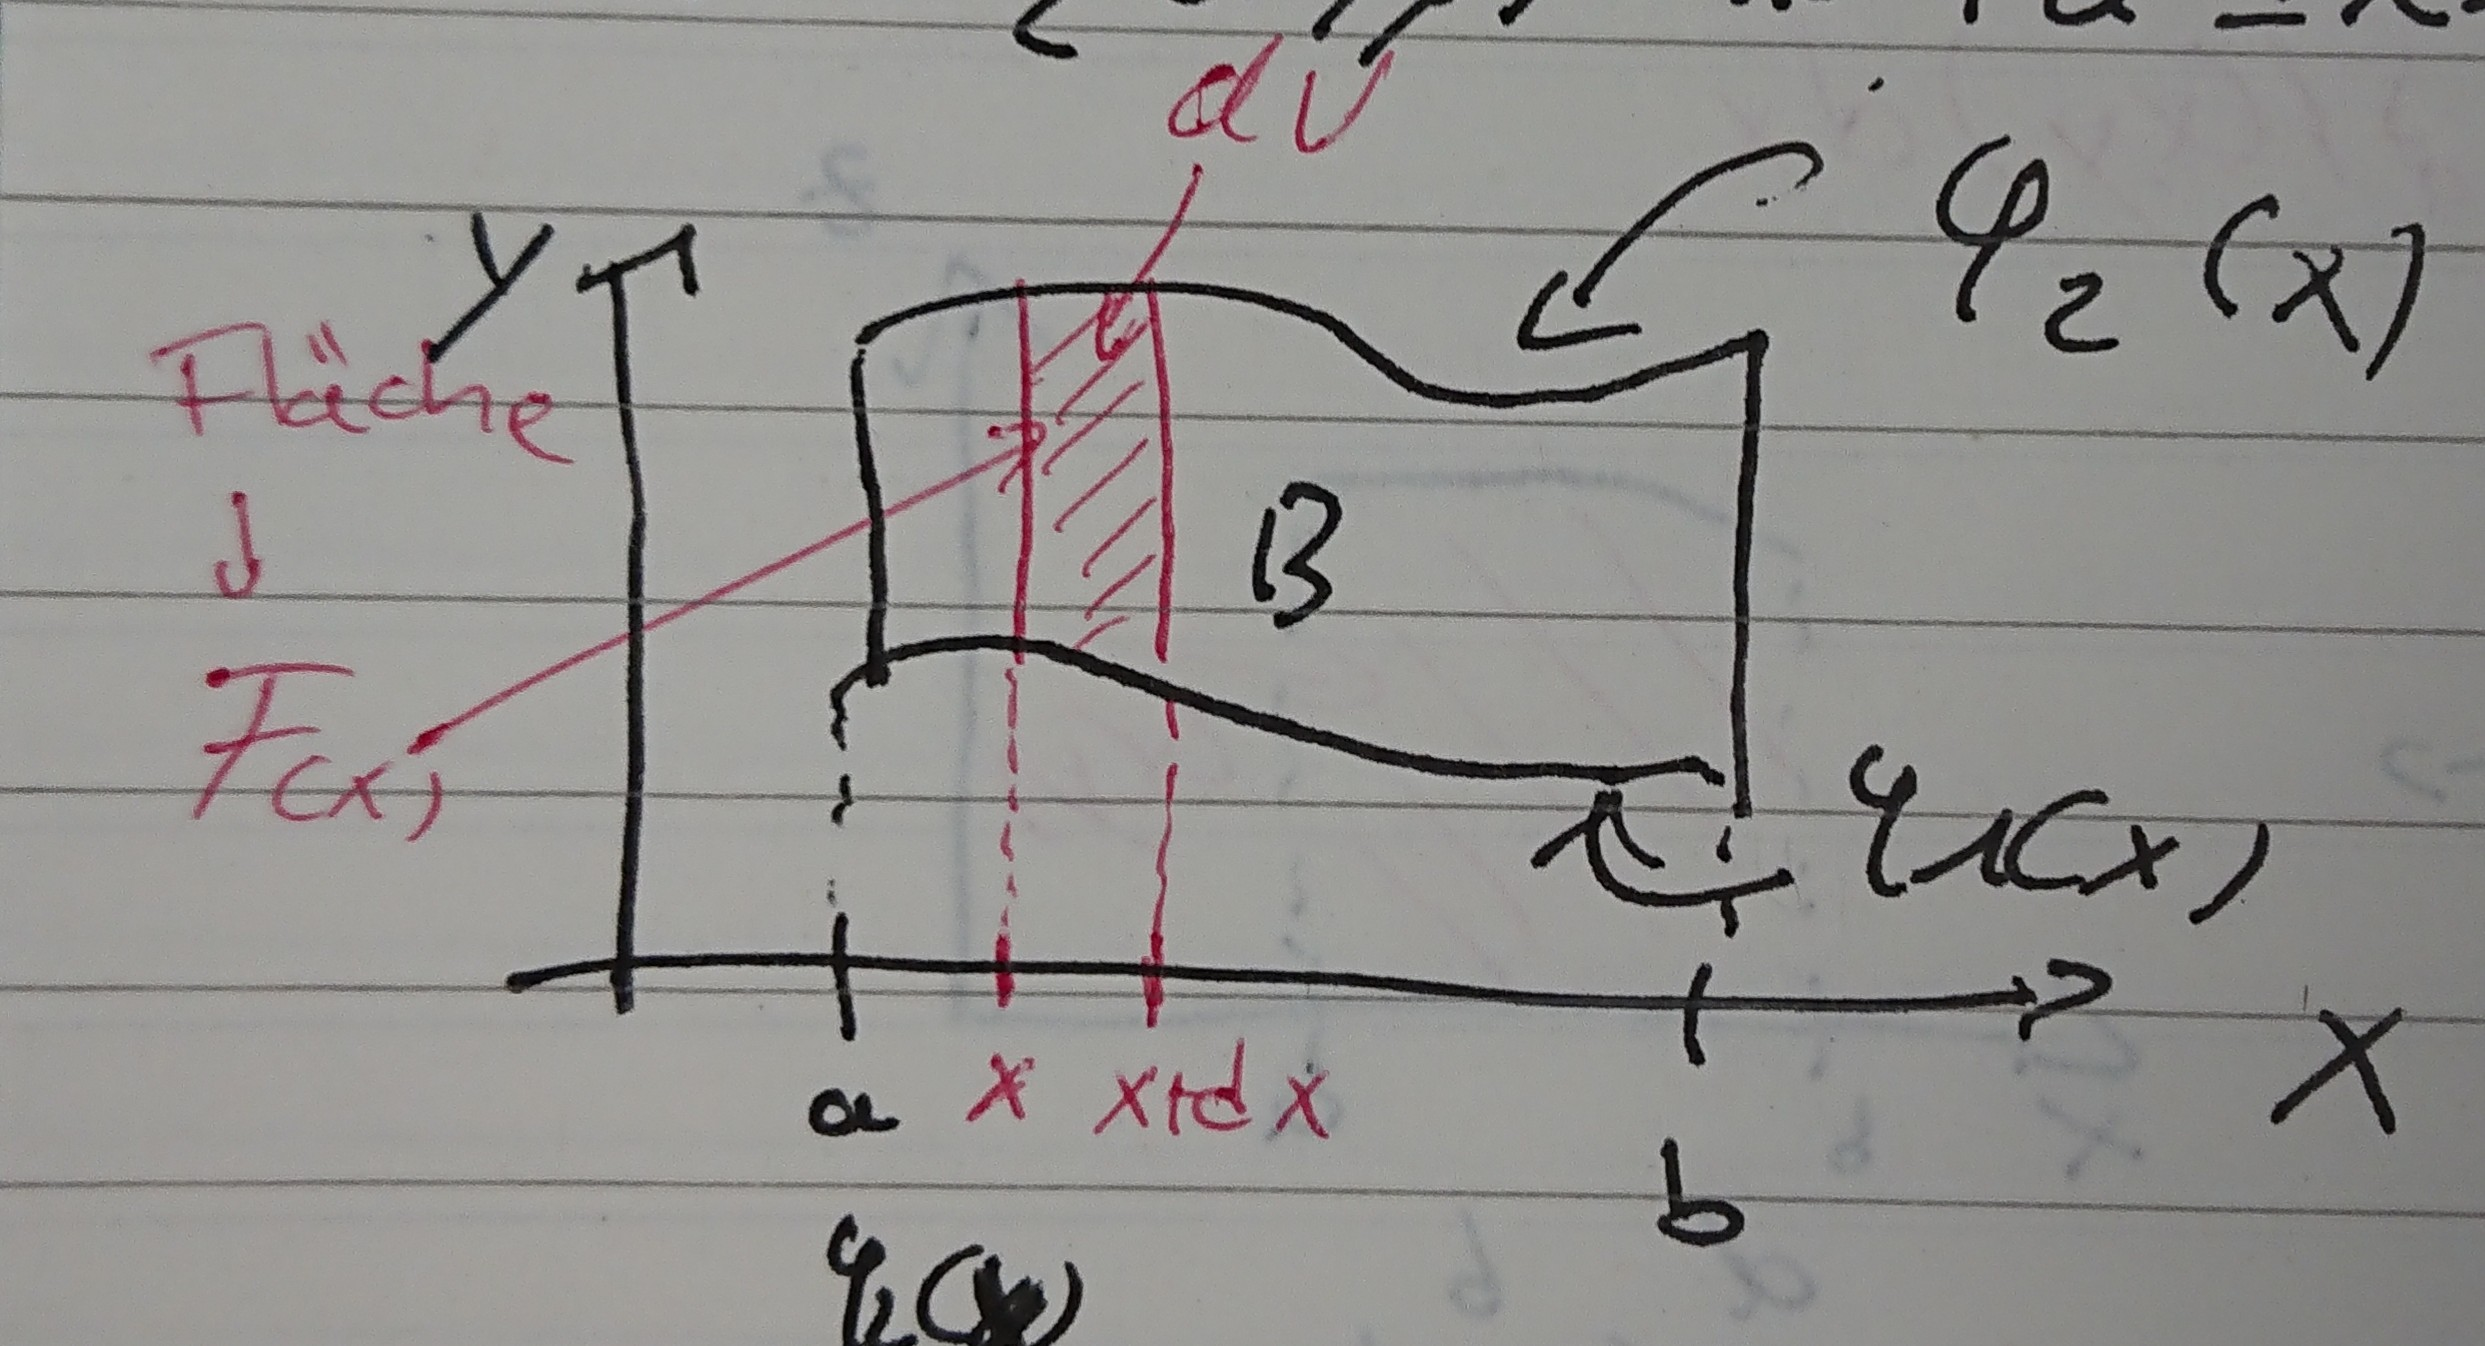
\includegraphics[width=0.5\textwidth]{./img/nb_typ1.jpg}
		  \caption{Normalbereich Typ I}
		  \label{fig:nb_typ1}
	  \end{figure}
	  \vspace{-0.5cm}
	  \begin{align}
	  	F(x) &= \int_{\varphi_1(x)}^{\varphi_2(x)} f(x,y) \dy \nonumber \\
	  	dV &= F(x) \dx \nonumber \\
	  	\Rightarrow V = \int_a^b F(x) \dx &= \int_a^b \int_{\varphi_1(x)}^{\varphi_2(x)}f(x,y) \dy \dx
	  \end{align}
	  
 	 \textbf{Normalbereich Typ $II$}
 	 \begin{equation}
 	 	B:= \lbrace (x,y) \in \R^2| \eta_1(x) \leq y \leq \eta_2(x), \; c \leq y \leq d\rbrace
 	 \end{equation}
	  \begin{figure}[H] 
		  \centering
		  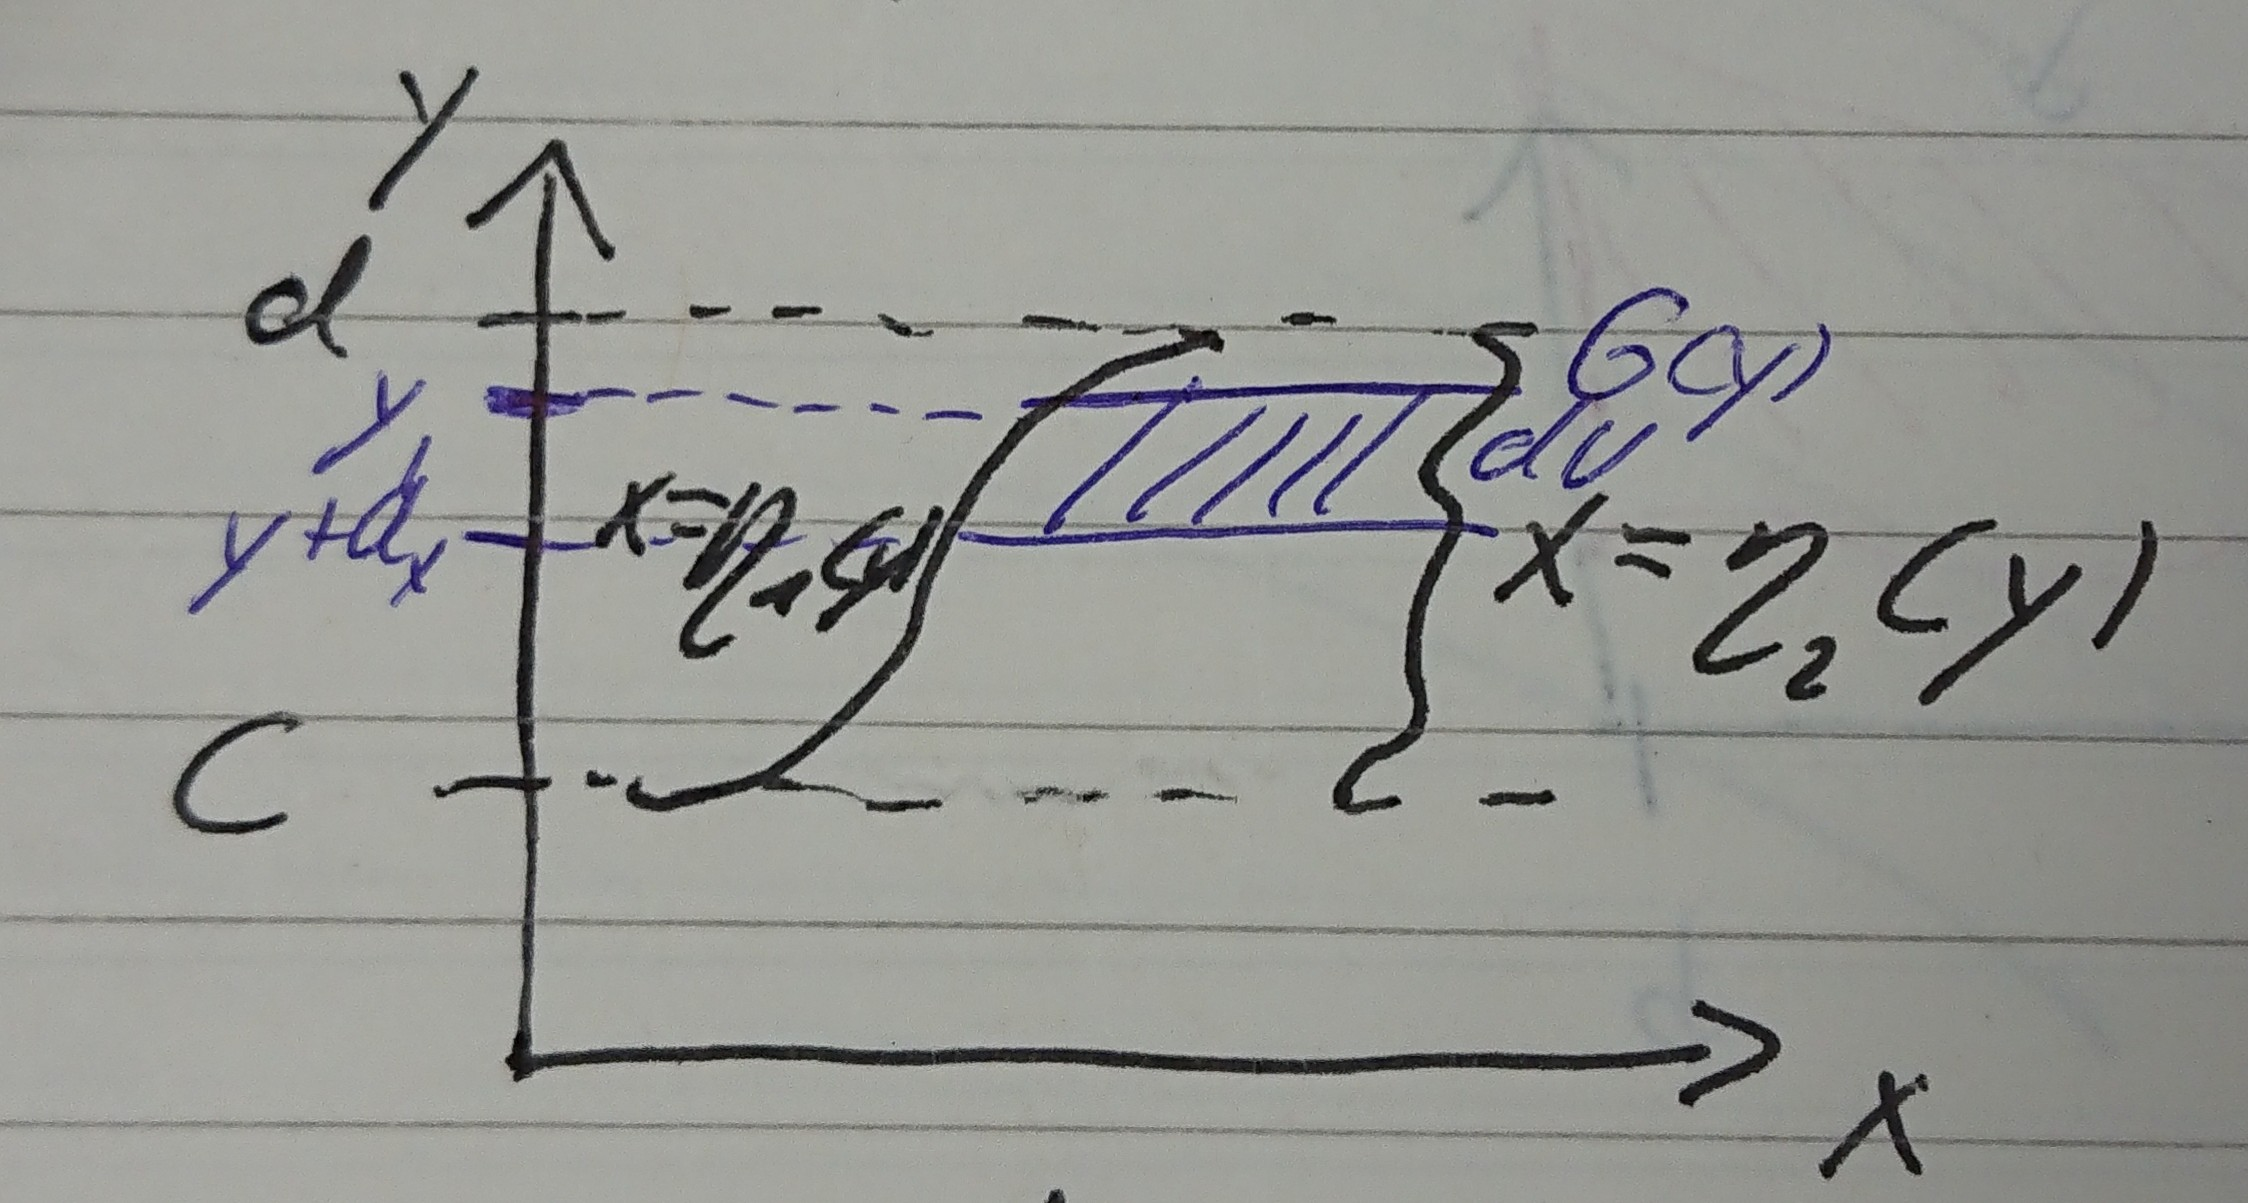
\includegraphics[width=0.5\textwidth]{./img/nb_typ2.jpg}
		  \caption{Normalbereich Typ II}
		  \label{fig:nb_typ2}
	  \end{figure}
	  \vspace{-0.5cm}
	  \begin{align}
	  	G(y) &= \int_{\eta_1(x)}^{\eta_2(x)} f(x,y) \dx \nonumber \\
	  	dV &= G(y) \dy \nonumber \\
	  	\Rightarrow V = \int_c^d G(y) \dy &= \int_c^d \int_{\eta_1(x)}^{\eta_2(x)}f(x,y) \dx \dy
	  \end{align}
 	 
 	  
	  \end{definition}
	  
	  